\chapter{Schriften}
\label{ch:Schriften}

Das grundlegende Arbeitsmittel der Typographie ist natürlich die
\emph{Schrift}.  Mit ihr wollen wir uns in diesem Kapitel umfassend
beschäftigen.  Einige Aspekte haben wir schon gesehen; hier gehen wir
aber weiter ins Detail.  Da sich die Gestaltung von Schrift »im
Kleinen« abspielt (im Gegensatz zur Gestaltung von bspw. ganzen
Seiten), wird das entsprechende Teilgebiet der Typographie auch als
\emph{Mikrotypographie} bezeichnet.

\section{Begriffliches und Klassifikation}

Eine \emph{Glyphe} ist die konkrete graphische Realisierung eines
(abstrakten) Schriftzeichens.  So sind bspw. \Char{a},
\Char{\textlarger{a}}, \Char{\textsmaller{a}}, \Char{\textit{a}},
\Char{\textbf{a}}, \Char{\textsf{a}}, \Char{\textsf{\textit{a}}} alles
unterschiedliche Glyphen, die den \emph{lateinischen Kleinbuchstaben
  a} darstellen.

Zusammenhängende Texte werden in einer \emph{Schriftart} gesetzt; die
darin vorhandenen Glyphen sind alle ähnlich und zueinander passend
gestaltet~-- sonst ergibt sich {U\fontfamily{ptm}\selectfont
  n\fontfamily{pplj}\selectfont r\fontfamily{lmr}\selectfont
  u\fontfamily{uop}\selectfont h\fontfamily{pcr}\selectfont e}.  Liegt
eine Schriftart in verschiedenen Varianten vor, was üblicherweise der
Fall ist, so werden diese \emph{Schriftschnitte} genannt (siehe
\cref{sec:Schnitte}).  Eine solche Schriftart mit mehreren Schnitten
nennt man dann auch eine \emph{Schriftfamilie}.\footnote{Das ist das
  Beste, was ich (Philip) nach längerer Recherche zur Unterscheidung
  der Begriffe \emph{Schriftart} und \emph{-familie} herausbekommen zu
  haben glaube.  Allerdings fällt mir spontan (während ich diesen Text
  schreibe) kein Beispiel für eine Schriftart ein, von der es nur
  einen Schnitt gibt, die also keine Familie ist.}

Schriftarten werden nach Aspekten ihrer Gestaltung klassifiziert.  Wir
beschäftigen uns hier nur mit \emph{Satzschriften} (also keine
Handschriften) für das lateinische Alphabet.  Diese werden
grundsätzlich unterschieden in zwei \emph{Schriftgattungen}, nämlich
\emph{Antiqua-Schriften}\footnote{Auch für das griechische, armenische
  und kyrillische Alphabet sind Antiqua-Schriften heutzutage üblich.}
einerseits und \emph{gebrochene Schriften} andererseits: in
gebrochenen Schriften haben die Bögen der Buchstaben »Knicke«; in
Antiqua-Schriften sind sie rund.  Heutzutage werden fast alle
Druckerzeugnisse im lateinischen Alphabet in Antiqua-Schriften
gesetzt, gebrochene Schriften (bspw. \emph{Textura},
\emph{Schwabacher}, \emph{Fraktur}) sind veraltet.

Historisch sind die Antiqua-Schriften im 15.\,Jahrhundert entstanden,
indem die Großbuchstaben der antiken \emph{Capitalis monumentalis}
--~der Schrift römischer Steininschriften~-- mit den Kleinbuchstaben
der \emph{humanistischen Minuskel} kombiniert wurden.  Für
handgeschriebene Bücher waren vorher reine Minuskelschriften üblich,
die sich ab Ende der Antike ursprünglich als Handschriften entwickelt
hatten; höchstens einzelne Anfangsbuchstaben wurden als ausgeschmückte
\emph{Initialen} in Großbuchstaben geschrieben.\footnote{Die
  englischen Bezeichnungen \emph{\foreignlanguage{british}{uppercase}}
  und \emph{\foreignlanguage{british}{lowercase}} für Groß-
  bzw. Kleinbuchstaben kommen aus der Zeit des Bleisatzes, als in
  Setzkästen die Lettern für Großbuchstaben in der oberen und die für
  Kleinbuchstaben in der unteren Schublade aufbewahrt wurden.}

\begin{figure}
  \centering
  \includegraphics[width=.4\textwidth]{Serifen}
  \caption{Schriftprobe \emph{(Liberation Serif)} mit markierten
    Serifen\protect\footnotemark}
  \label{fig:Serifen}
\end{figure}
\footnotetext{Autor:
  \href{https://commons.wikimedia.org/wiki/File:Serif_and_sans-serif_03.svg}
  {XRDoDRX auf Wikimedia Commons},
  Lizenz: \href{https://creativecommons.org/licenses/by-sa/3.0/}
  {\acr{CC BY-SA}\,3.0}}

Innerhalb der Gattung der Antiqua-Schriften werden Schriftarten weiter
in kleineren »Taxa« (um mal ein Wort aus der Biologie
zweckzuentfremden) klassifiziert:\footnote{In der Zeit des Bleisatzes
  war in Deutschland die Klassifikation gemäß \acr{DIN}~16518 üblich
  (siehe \url{https://de.wikipedia.org/wiki/DIN_16518}); diese ist
  aber einerseits kunsthistorisch fragwürdig und andererseits
  veraltet.  Wir orientieren uns im Folgenden grob an der Matrix
  Beinert (siehe
  \url{https://www.typolexikon.de/schriftklassifikation-matrix-beinert/}).}
Die Gattung wird unterteilt in \emph{Hauptschriftgruppen} und diese
jeweils in \emph{Schriftuntergruppen}.  Die Hauptschriftgruppen
unterscheiden sich dabei durch die Art der an den Glyphen vorhandenen
\emph{Serifen}, den Linien, die die Hauptstriche »abschließen« (siehe
\cref{fig:Serifen}).  Die Klassifikation ist wie folgt:
\begin{itemize}
\item Eine Schrift mit »normalen«, nicht betonten Serifen heißt
  \emph{Antiqua} bzw. englisch \emph{\foreignlanguage{british}{serif}}
  oder \emph{\foreignlanguage{british}{roman}} (ja, der Name der
  Hauptschriftgruppe ist derselbe wie der der Gattung; diese
  Schriftarten waren nämlich die ursprünglichen Antiqua-Schriften).
  Nach ihrem historischen Entstehungszeitpunkt werden die folgenden
  drei Schriftuntergruppen unterschieden:
  \begin{itemize}
  \item \emph{Renaissance-Antiqua}, mit den Schriftnebengruppen
    \emph{Venezianische} und \emph{Französische Renaissance-Antiqua}:
    bspw. {\fontfamily{EBGaramond-OsF}\selectfont Garamond},
    {\fontfamily{pplj}\selectfont \textsmaller[.5]{Palatino}}, % URW Palladio L 
    Minion
  \item \emph{Vorklassizistische Antiqua}\footnote{Nach
      \acr{DIN}~16518: »Barock-Antiqua« (irreführend)}:
    bspw. {\fontfamily{Baskervaldx-OsF}\selectfont Baskerville},
    {\fontfamily{ptm}\selectfont Times} % Nimbus Roman No. 9 L
  \item \emph{Klassizistische Antiqua}:
    bspw. {\fontfamily{bodoni}\selectfont Bodoni},
    {\fontfamily{TheanoDidot-TOsF}\selectfont Didot},
    {\fontfamily{lmr}\selectfont Computer Modern / Latin Modern}
  \end{itemize}
\item Eine Schrift mit betonten Serifen heißt \emph{Egyptienne} bzw.
  englisch \emph{\foreignlanguage{british}{slab serif}}.\footnote{Nach
    \acr{DIN}~16518: »Serifenbetonte Linear-Antiqua«}
  (Schriftuntergruppen sind uns hier egal.)  Bspw.
  {\fontfamily{bch}\selectfont Bitstream Charter},
  {\fontfamily{ccr}\selectfont Concrete Roman},
  {\fontfamily{ucr}\selectfont Courier} % Nimbus Mono L
\item Eine Schrift ohne Serifen heißt \emph{Grotesk} bzw. englisch (ja
  ja, mit Französisch) \emph{\foreignlanguage{british}{sans
      serif}}.\footnote{Nach \acr{DIN}~16518: »Serifenlose
    Linear-Antiqua«} (Auch hier sind uns Schriftuntergruppen egal.)
  Bspw.  {\fontfamily{phv}\selectfont \textsmaller[.5]{Helvetica}}, % Nimbus Sans L
  {\fontfamily{pag}\selectfont \textsmaller[.5]{Avant Garde}}, % Gothic L
  {\fontfamily{ua1}\selectfont \textsmaller[.5]{Arial}} % URW A030
\item Die letzte Hauptschriftgruppe der Antiqua-Schriften sind
  \emph{Zierschriften}.  Das sind generell alle Antiqua-Schriften, die
  keine Antiqua, Egyptienne oder Grotesk sind. Zu ihnen gehören
  u.\,a. die sog. \emph{Antiqua-Varianten} nach \acr{DIN}~16518.  Ein
  Beispiel für letztere sind sog. \emph{Inzisen}, an Inschriften
  orientierte Schriften mit sehr dezenten Serifen, wie bspw.
  \textsf{\textsmaller[.5]{Optima / Classico}}.\footnote{Die Optima
    wird gerne --~so auch in diesem Skript~-- als Grotesk zu Palatino
    oder Minion verwendet, obwohl sie eigentlich™ keine ist.}
\end{itemize}
Die Gestaltung und Klassifikation von Schriften gleicht einem Fass
ohne Boden; wir gehen hier nicht weiter ins Detail.\footnote{Wer
  möchte, kann dazu sehr viel Weitergehendes auf Wikipedia oder im
  Typo\-lexikon (\url{https://www.typolexikon.de/}) lesen.}

Die Schrift, in der der Großteil eines typographischen Werks gesetzt
wird, wird historisierend die jeweilige \emph{Brotschrift} genannt~--
mit ihr haben Schriftsetzer früher »ihr täglich Brot« verdient.
Angeblich™ lesen sich im Fließtext Schriften mit Serifen leichter als
Grotesken.  Es gibt dazu auch einige Untersuchungen; soweit ich
(Philip) weiß, sind die aber zu keinen aussagekräftigen (sprich
statistisch signifikanten) Ergebnissen gekommen.  (Tatsächlich sind
serifenlose Schriften wohl teilweise hilfreich bei Legasthenie.)  Auf
jeden Fall sind Grotesken eine jüngere Erfindung (sie sind Anfang des
19.\,Jahrhunderts entstanden), und »traditionell« werden gedruckte
Fließtexte in Antiqua gesetzt.  Besonders bei (hochqualitativen)
Büchern sind Renaissance-Antiquas üblich.  Auf nicht allzu hoch
aufgelösten Pixel-Bildschirmen sind Serifen oft eher schlecht in
gleichmäßiger Qualität darstellbar; daher werden in
Computer-Kontexten, bspw. im Webdesign, häufig auch serifenlose
Schriften als Brotschrift eingesetzt.

\section{Schriftschnitte}
\label{sec:Schnitte}

Die verschiedenen Schriftschnitte einer Schriftfamilie unterscheiden
sich üblicherweise in den \emph{Auszeichnungsmerkmalen}
\begin{itemize}
\item \emph{Schriftstärke},
\item \emph{Schriftlage} und
\item \emph{Schriftbreite}.
\end{itemize}
Grundsätzlich können Ausprägungen der verschiedenen Merkmale frei
miteinander kombiniert werden; ob eine konkrete Schriftfamilie den
entsprechenden Schnitt hat ist eine andere Frage (und ebenso, ob und
wann man »merkwürdige« Schnitte einsetzen möchte).

Die \emph{Schriftstärke} bezeichnet die Dicke der Striche, aus denen
die Glyphen bestehen.  Es gibt üblicherweise mindestens die
Schriftstärken \emph{normal}
(engl. \emph{\foreignlanguage{british}{regular}}) und \emph{fett}
(engl. \emph{\foreignlanguage{british}{bold}}); viele Schriftfamilien
bieten aber auch Zwischenstufen (siehe \cref{fig:Schriftstärken}).
Die Schriftstärke hat einen Einfluss auf den \emph{Grauwert} der
Schrift: stärkere Glyphen wirken dunkler.

\begin{figure}
  \centering
  \includegraphics[width=.5\textwidth]{Schriftstärken}
  \caption{Verschiedene Schriftstärken \emph{(Helvetica Neue)}}
  \label{fig:Schriftstärken}
\end{figure}

Die \emph{Schriftlage} gibt an, ob die Glyphen »aufrecht« stehen oder
»geneigt« sind; üblicherweise wird unterschieden zwischen
\emph{normal} (engl. \emph{\foreignlanguage{british}{roman}}) und
\emph{kursiv} engl. \emph{\foreignlanguage{british}{italic}}.
Historisch geht kursive Schrift auf Schreibschriften (»Kursive«)
zurück, konkret auf die \emph{humanistische Kursive} von \name{Niccolò
  de' Niccoli} (1364--1437).  Daher ändert sich von normaler zu
kursiver Schrift meist --~zumindest bei Antiqua~-- auch die Form der
Buchstaben.  Wie schon in \cref{sec:herv_kursiv} erwähnt sollte man
deshalb vermeiden, kursive Schrift durch künstlich geschrägte Schrift
(engl. \emph{\foreignlanguage{british}{slanted}}) zu ersetzen.  Bei
Grotesken ist der kursive Schnitt meist aber tatsächlich vor allem
geneigt, ohne die Form der Glyphen zu verändern.\footnote{Manche
  Schriftfamilien unterscheiden zwischen den Lagen \emph{kursiv} und
  \emph{schräg} (engl. \emph{\foreignlanguage{british}{oblique}}); das
  ist aber ziemlich selten.}  Ein Beispiel findet sich in
\cref{fig:Schriftlagen}.  Schriftschnitte in verschiedenen Lagen sind
üblicherweise so gestaltet, dass der Grauwert unverändert ist.

\begin{figure}
  \centering

  \subfloat[\emph{Minion}]
  {\begin{minipage}{.35\textwidth}
      \large Minion normal afg

      \textit{Minion kursiv afg}

      \textsl{Minion geschrägt afg}\par
    \end{minipage}}
  \hspace{.1\textwidth}
  \subfloat[\emph{Classico}]
  {\begin{minipage}{.35\textwidth}
      \large\sffamily Classico normal afg

      \textit{Classico kursiv afg}

      \textsl{Classico geschrägt afg}\par
    \end{minipage}}

  \caption{Verschiedene Schriftlagen}
  \label{fig:Schriftlagen}
\end{figure}

Schließlich gibt es noch Schriftfamilien, bei denen die
\emph{Schriftbreite} variiert werden kann.  Außer einer
\emph{normalen} Breite
(engl. \emph{\foreignlanguage{british}{regular}}) gibt es dann
bspw. die Breiten \emph{schmal}
(engl. \emph{\foreignlanguage{british}{condensed}}) oder \emph{breit}
(engl. \emph{\foreignlanguage{british}{expanded}}), manchmal auch in
\emph{halb-} (engl. \emph{\foreignlanguage{british}{semi}}),
\emph{extra-} oder gar \emph{ultra-}.  Ein Beispiel findet sich in
\cref{fig:Schriftbreiten}.

\begin{figure}
  \centering
  \includegraphics[width=.5\textwidth]{Schriftbreiten}
  \caption{Schriftbreiten \emph{normal} und \emph{schmal}
    (\emph{Avenir Next}, Schrifstärke \emph{Demi-Bold})}
  \label{fig:Schriftbreiten}
\end{figure}

Abgesehen von den oben erwähnten üblichen Auszeichnungsmerkmalen haben
gute Schriften meist noch Schriftschnitte für \emph{Kapitälchen}
(siehe \cref{sec:Kapitälchen}).  Außerdem gibt es bei professionellen
Schriften oft verschiedene \emph{optische Größen}, d.\,h. Schnitte,
die an verschiedene Schriftgrößen angepasst sind (siehe
\cref{fig:optische_Größen}).

\begin{figure}
  \centering
  \includegraphics[width=.65\textwidth]{optische_Größen}
  \caption{Verschiedene optische Größen \emph{(Minion
      Pro)}\protect\footnotemark}
  \label{fig:optische_Größen}
\end{figure}
\footnotetext{Autor:
  \href{https://www.typolexikon.de/konsultationsgroessen/optische-groessen-optical-sizes/}
  {Wolfgang Beinert},
  \href{https://www.typolexikon.de/}{www.typolexikon.de}}

\section{Schriftlinien und Maßeinheiten}
\label{sec:Linien}

Die \emph{metrische} Gestaltung einer Schrift, also die Größe ihrer
Glyphen und der Teilbestandteile der Glyphen, wird mithilfe von
\emph{Schriftlinien} beschrieben (siehe \cref{fig:Liniensystem}).  Die
Glyphen ruhen auf der \emph{Grundlinie}.  Großbuchstaben reichen nach
oben bis zur \emph{H-Linie}; die Höhe der Großbuchstaben wird als
\emph{Versalhöhe} bezeichnet.  Für Kleinbuchstaben spielen insgesamt
vier Linien eine Rolle: zusätzlich zur Grundlinie sind das die
\emph{x-Linie}, bis zu der die \emph{Mittellänge} (das »mittlere
Stockwerk«) der Buchstaben reicht, die \emph{p-Linie}, zu der
Buchstaben mit \emph{Unterlänge} (einem »unteren Stockwerk«)
herabreichen, und die \emph{k-Linie}, zu der Buchstaben mit
\emph{Oberlänge} (einem »oberen Stockwerk«) hinaufreichen.  Der
Abstand von Grundlinie zu x-Linie heißt \emph{x-Höhe}.  (Relevant für
die Schriftgestaltung ist außerdem noch die \emph{Á-Linie}, bis zu der
Akzente auf Majuskeln reichen.)  Die entsprechenden Teile der Glyphen
hören oft nicht strikt an den entsprechenden Linien auf, insbesondere
bei Rundungen; stattdessen ragen sie oft ein bisschen über, sodass sie
\emph{optisch} »an der Linie« enden.  Zu beachten ist noch, dass es
eine eigene k-Linie \emph{nur bei Renaissance-Antiquas} gibt; bei
allen anderen Antiqua-Schriften reichen Oberlängen von Minuskeln wie
die Majuskeln bis zur \mbox{H-Linie}.

\begin{figure}
  \centering
  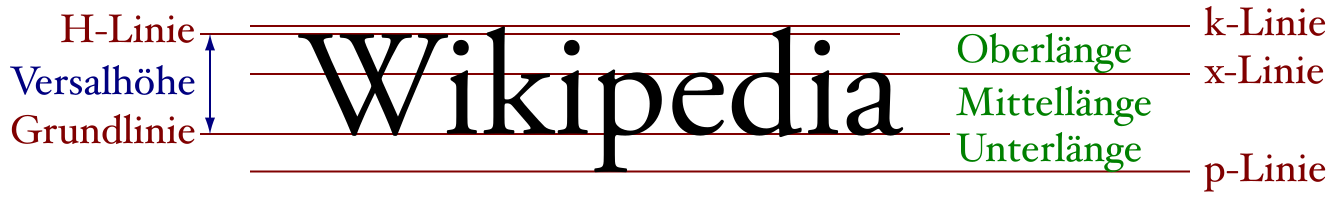
\includegraphics[width=\textwidth]{Liniensystem}
  \caption{Schriftlinien\protect\footnotemark}
  \label{fig:Liniensystem}
\end{figure}
\footnotetext{Modifiziert nach
  \href{https://de.wikipedia.org/wiki/Datei:Typografisches_Liniensystem.svg}
  {Crissov auf Wikipedia},
  Lizenz: \href{https://creativecommons.org/licenses/by-sa/4.0/}
  {\acr{CC BY-SA}\,4.0}}

Die grundlegende Maßeinheit für Längen in der Typographie ist der
\emph{typographische Punkt}, von dem es historisch verschiedene
Versionen gab und gibt.  Heutzutage üblich ist der
\emph{Desktop-Publishing-Punkt} \emph{(\acr{DTP}-Punkt)}: er ist
definiert als 1\,pt = \smallfrac{1}{72}\,in =
0,352$\overline{\text{7}}$\,mm.  In Punkt wird die \emph{Schriftgröße}
(bzw. der \emph{Schriftgrad}) angegeben.  Zur Zeit des Bleisatzes war
das die \emph{Kegelstärke} (bzw. \emph{Kegelhöhe}) der Lettern (siehe
\cref{fig:Bleiletter}).  Im Foto- und besonders im Digitalsatz ist die
Angabe von Schriftgrößen zwar weiter grob am historischen Vorbild
orientiert, aber verschiedene Schriften desselben Schriftgrades können
optisch deutlich verschieden groß wirken.  Als (sehr) grobe Faustregel
kann man sich merken, dass die Versalhöhe einer Schrift ca. 70--75\,\%
und die x-Höhe ca. 45--50\,\% des Schriftgrades beträgt.

\begin{figure}
  \centering
  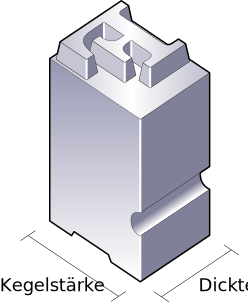
\includegraphics[width=.5\textwidth]{Bleiletter}
  \caption{Bleiletter}
  \label{fig:Bleiletter}
\end{figure}

Ist eine Schriftgröße festgelegt, so nennt man die entsprechende Länge
ein \emph{Geviert}.  Historisch kommt dieser Name von quadratischen
nicht druckenden Lettern (»Geviert« ist ein veraltetes Wort für
»Quadrat«): ein Geviert war ein Letter, der so breit war wie die
Kegelstärke.  Entsprechend benennt man Anteile dieser Länge bspw. als
\emph{Halb-} oder \emph{Viertelgeviert}~-- daher auch die
typographischen Namen der verschiedenen Striche
(vgl. \cref{sec:Striche}).  Auf Englisch heißt das Geviert
\emph{\foreignlanguage{british}{quad}} oder
\emph{\foreignlanguage{british}{em}}, das Halbgeviert
\emph{\foreignlanguage{british}{en}}.\footnote{Manchmal wird
  behauptet, das komme daher, dass die Großbuchstaben \Char{M}
  bzw. \Char{N} die entsprechende Breite haben.  Das ist aber falsch:
  Üblicherweise ist ein \Char{M} ein wenig schmaler als ein Geviert.}

%% Zeilenabstand: eigentlich sollte™ man einfach den Abstand zwischen
%% den Grundlinien messen.  Es gibt sinnvolle Standardeinstellungen,
%% bspw. in LaTeX 10pt → 12pt, 11pt → 13.6pt, 12pt → 14.5pt.  MS Word
%% und LibreOffice benutzen auch ca. 1,2-faches der Schriftgröße als
%% Grundeinstellung, das heißt da aber »einzeilig«.

\section{Spationierung und Unterschneidung}

%% Hier microtype erwähnen?

\section{Ligaturen}

%% Ligatur = eine Glyphe für mehrere Buchstaben.  Sinnvoll, um
%% ruhigeres Schriftbild zu erreichen.  Traditionelle Ligaturen aus
%% lateinischen Texten; je nach Sprache zusätzliche.  Fun fact: ß =
%% ſ-z- oder ſ-s-Ligatur.  (Problem: die Minion hat kein ſ :( )

%% Ligaturbrecher erwähnen!

\section{Ziffern}
\label{sec:Ziffern}

%% Minuskelziffern, Majuskelziffern, Tabellenziffern / lining figures

\section{Beispiele}

{\fontfamily{pplj}\selectfont Palatino 1234 \emph{kursiv} \textsc{kapitälchen}}
%% Garamond, Palatino, Minion, Optima/Classico, Times, Helvetica

%% Jeweils auch die lustigen Namen nach DIN 16518 erwähnen!

%%% Local Variables:
%%% mode: latex
%%% TeX-master: "main"
%%% End:
